\chapter{Design}

\section{Analysis of an image}

\subsection{Using Harris corner detector}
The analysis of an image begins with applying the Harris detector on it. It will compute a given score for each pixel of the image, the higher the score, the greater the chance that pixel represents a corner.\\
Using these values we will have to determine a subset of pixels that will represent the Harris mask of the image. Experimentally, I have established that all the points which have a value greater than $0.01 * max\_image\_value$ are to be part of the subset.\\
As an example, Figure~\ref{fig:beforeHarris} shows a normal image of a woman's face, while Figure~\ref{fig:afterHarris} shows the corresponding pixels that form the corner mask. \\

\begin{figure}[ht!]
\centering
\begin{minipage}{.5\textwidth}
	\centering
	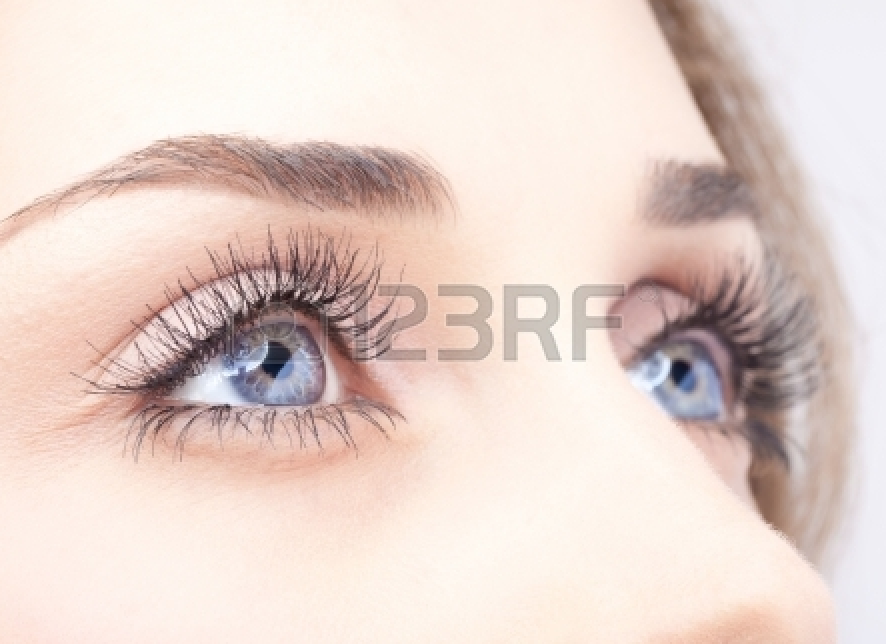
\includegraphics[width=.8\linewidth]{images/beforeHarris.png}
	\caption{Sample image}
	\label{fig:beforeHarris}
\end{minipage}%
\begin{minipage}{.5\textwidth}
	\centering
	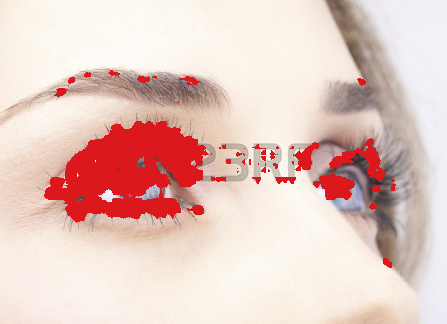
\includegraphics[width=.8\linewidth]{images/afterHarris.png}
	\caption{Harris corner mask applied }
	\label{fig:afterHarris}
\end{minipage}
\end{figure}

As it can be seen from the image, the corner mask centers around the interest points in the image, the eyes and the eyelashes, while leaving the smooth surfaces (the skin) unmarked.

Another observation is that possible watermarks can be present in the image (as seen above), which, of course, the mask detects (they are center pieces of the image, and the corner algorithm cannot determine that they have no real connection with the image).

Furthermore, in some cases the watermark might contain all the points in the mask (as seen in Figure~\ref{fig:watermarkHarris}). To avoid such a behavior, the image is split into 9 sub images (three rows and three columns of identical dimensions) and the Harris mask is applied to each of these.

\begin{figure}[ht!]
\centering
\begin{minipage}{.5\textwidth}
	\centering
	
\includegraphics[width=.8\linewidth]{images/watermarkHarris.png}
	\caption{Single image}
	\label{fig:watermarkHarris}
\end{minipage}%
\begin{minipage}{.5\textwidth}
	\centering
	
\includegraphics[width=.8\linewidth]{images/watermarkHarris9.png}
	\caption{9 subimages}
	\label{fig:watermarkHarris9}
\end{minipage}
\end{figure}

This determines the corner mask to also contain pixels from the center of the image (some of which, unfortunately, are also a watermark).


\subsection{Using SIFT keypoints and descriptors}

As we have seen, in ceva, the SIFT algorithm computes the keypoints of an image, and then computes descriptors for these keypoints. Due to the high similarity nature of our problem, we do not want to compute the keypoints for the entire image, but filter them based on the corner mask determined in the previous section (as observed in Figure~\ref{fig:messiSift} and Figure~\ref{fig:messiCornerSift})

\begin{figure}[ht!]
\centering
\begin{minipage}{.5\textwidth}
	\centering
	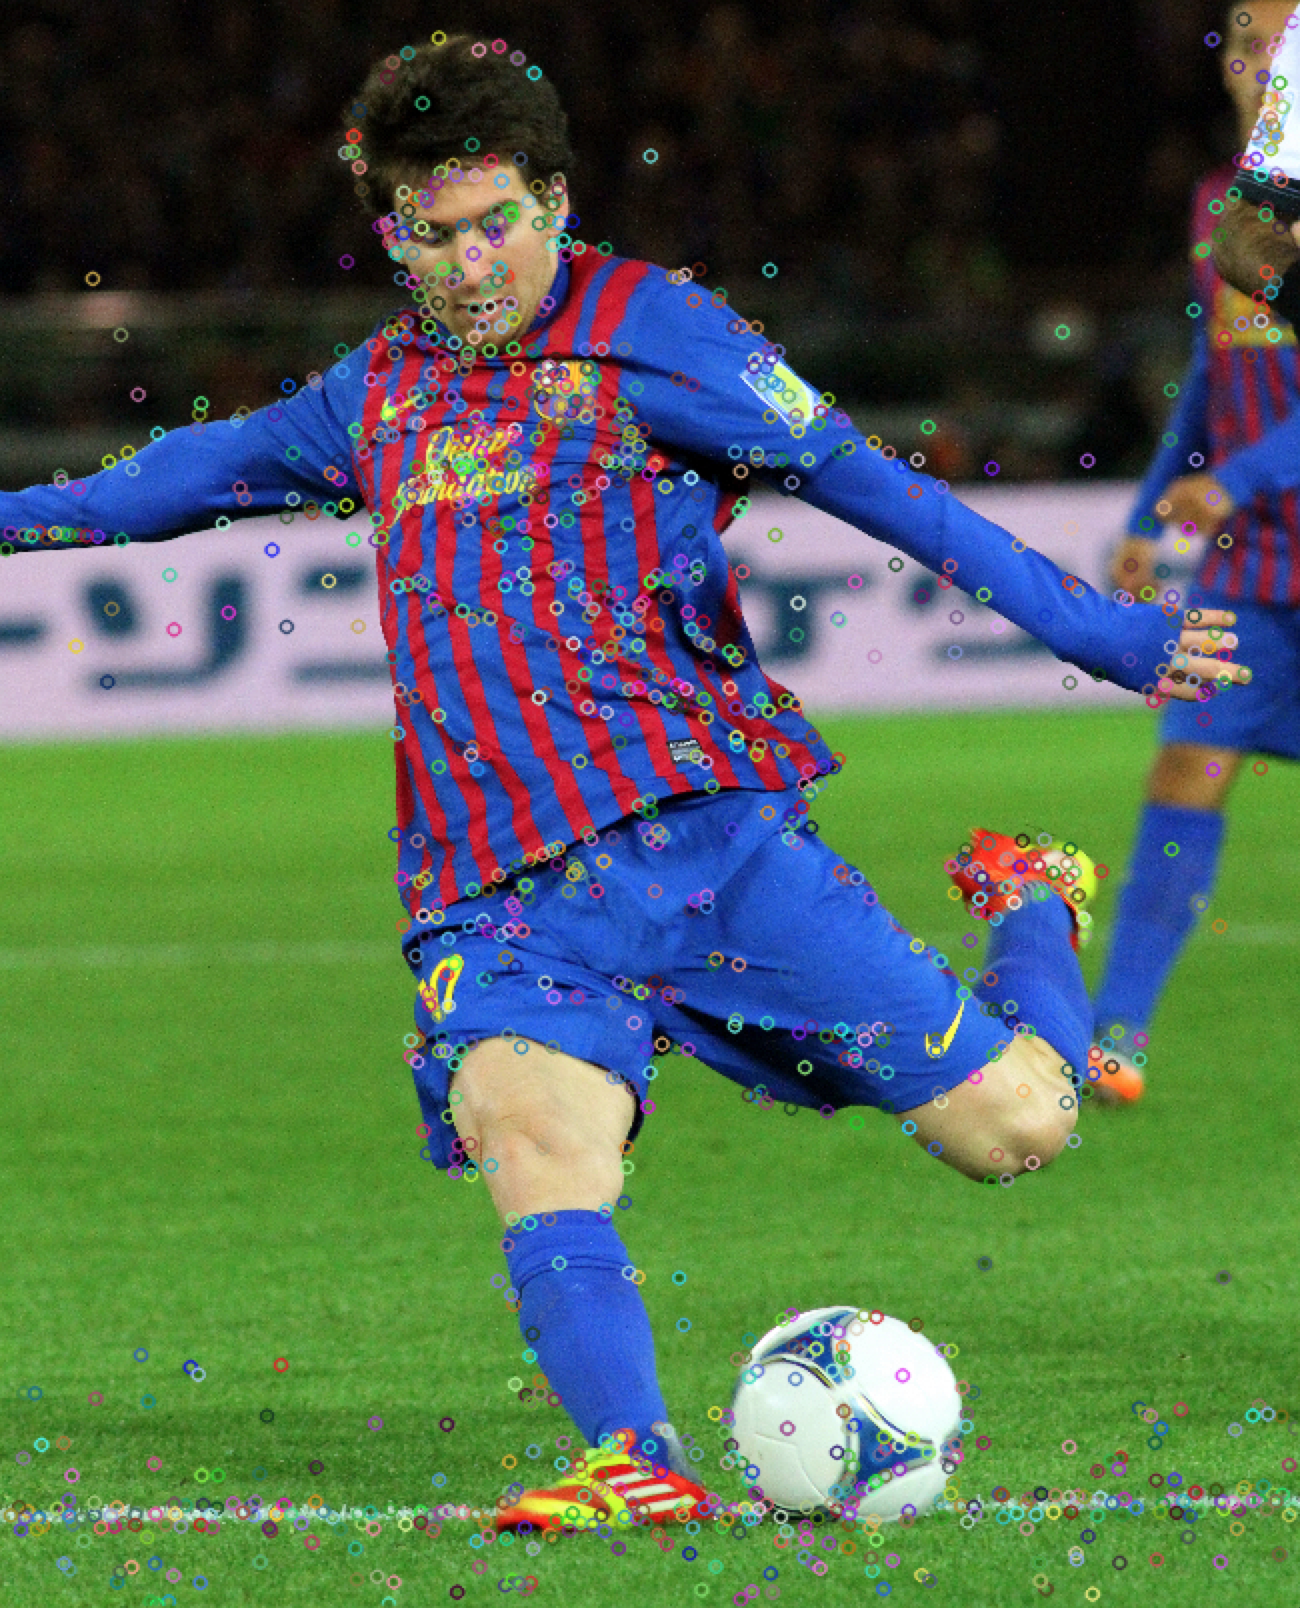
\includegraphics[width=.8\linewidth]{images/messiSift.png}
	\caption{SIFT keypoints for the\\ entire image}
	\label{fig:messiSift}
\end{minipage}%
\begin{minipage}{.5\textwidth}
	\centering
	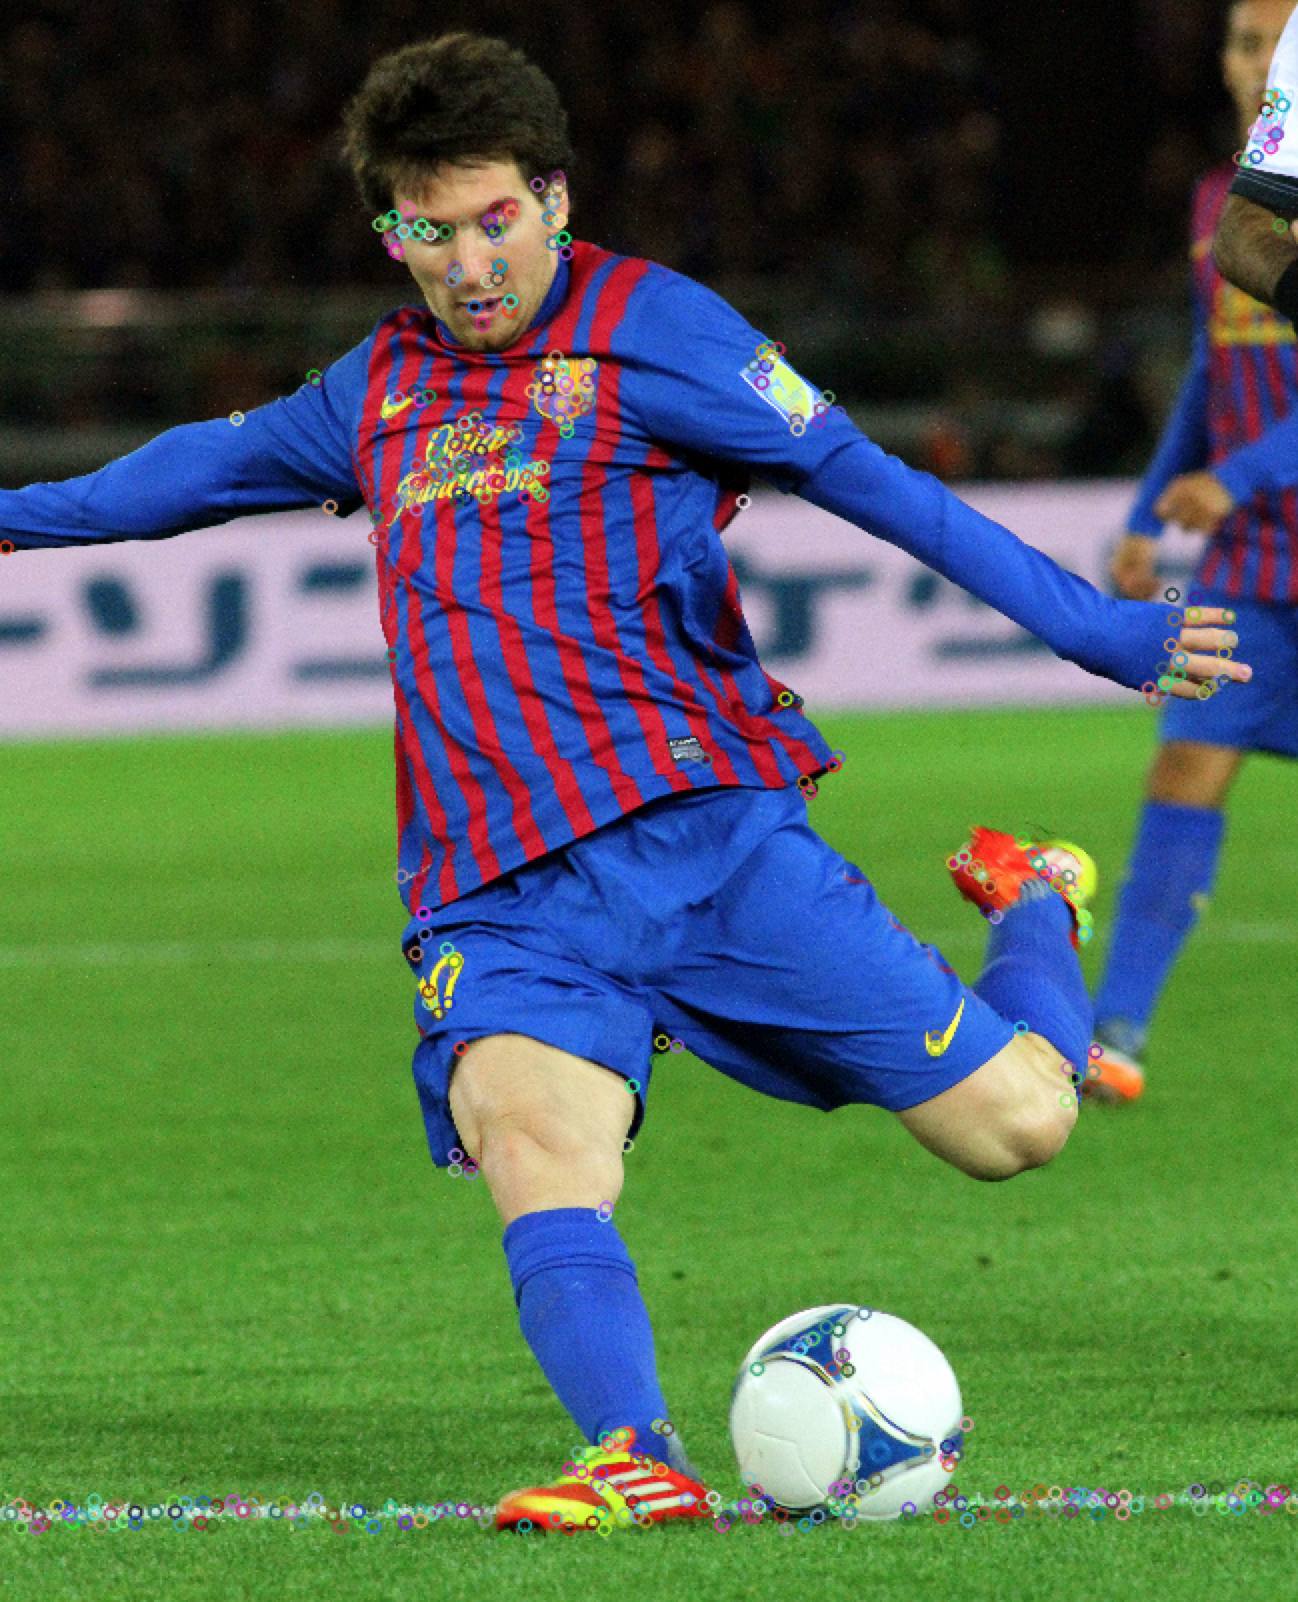
\includegraphics[width=.8\linewidth]{images/messiCornerSift.png}
	\caption{SIFT keypoints for corner mask}
	\label{fig:messiCornerSift}
\end{minipage}
\end{figure}

The SIFT descriptors are then computed for each keypoint located in the corner mask and this will be the information stored for a certain image.

\section{Analysis of a pair of images}
